\documentclass[11pt,a4paper]{article}

\usepackage[utf8]{inputenc}
\usepackage[T1]{fontenc}
\usepackage[margin=2.4cm]{geometry}
\usepackage{amsmath,amssymb,amsthm,mathtools}
\usepackage{booktabs,array,enumitem}
\usepackage{xcolor}
\usepackage{tikz}
\usetikzlibrary{arrows.meta,calc,positioning,decorations.markings}
\usepackage{pgfplots}
\usepackage{float}
\pgfplotsset{compat=1.16}
\usepackage[most]{tcolorbox}
\usepackage[colorlinks=true,linkcolor=blue!50!black,urlcolor=blue!50!black]{hyperref}

% ---------- macros ----------
\newcommand{\q}{\boldsymbol{q}}
\newcommand{\qi}{\boldsymbol{q}_i}
\newcommand{\qf}{\boldsymbol{q}_f}
\newcommand{\ut}{\tilde{\boldsymbol{u}}}
\newcommand{\vt}{\tilde v}
\newcommand{\wt}{\tilde\omega}
\newcommand{\wwt}{\tilde w}
\newcommand{\dd}{\mathrm{d}}
\newcommand{\sign}{\operatorname{sign}}
\newcommand{\atan}{\operatorname{atan2}}
\newcommand{\Null}{\mathcal{N}}

% ---------- theorem-like environments (amsthm, boxed) ----------
\theoremstyle{definition}
\newtheorem{definition}{Definition}[section]
\newtheorem{example}[definition]{Example}
\newtheorem{algorithm}[definition]{Algorithm}
\theoremstyle{plain}
\newtheorem{theorem}[definition]{Theorem}
\newtheorem{lemma}[definition]{Lemma}
\newtheorem{proposition}[definition]{Proposition}
\newtheorem{corollary}[definition]{Corollary}
\theoremstyle{remark}
\newtheorem*{remark}{Remark}

\tcbset{thmbox/.style={enhanced,breakable,colback=gray!4,colframe=black!55,boxrule=0.5pt,
  arc=1.5pt,left=6pt,right=6pt,top=4pt,bottom=4pt,before skip=8pt,after skip=8pt}}
\tcolorboxenvironment{definition}{thmbox}
\tcolorboxenvironment{theorem}{thmbox}
\tcolorboxenvironment{lemma}{thmbox}
\tcolorboxenvironment{proposition}{thmbox}
\tcolorboxenvironment{corollary}{thmbox}
\tcolorboxenvironment{example}{thmbox}
\tcolorboxenvironment{algorithm}{thmbox}

% ---------- blue Intuition box ----------
\newtcolorbox{intuition}{enhanced,breakable,colback=blue!5,colframe=blue!60!black,
  coltitle=white,fonttitle=\bfseries,title={Intuition},boxrule=0.6pt,arc=2pt,
  left=6pt,right=6pt,top=4pt,bottom=4pt,before skip=8pt,after skip=10pt}

\title{\textbf{Autonomous and Mobile Robotics}\\[2pt]
\large Wheeled Mobile Robots: Path \& Trajectory Planning\\[2pt]
\normalsize Lecture notes}
\author{}
\date{}

\begin{document}
\maketitle
\tableofcontents
\bigskip

\noindent\textbf{Roadmap.} The lecture is about computing motions for a wheeled mobile robot (WMR) that
\emph{respect its nonholonomic constraints}, in free space (no obstacles). The plan is:
separate space from time; characterize which \emph{paths} are admissible (geometric model);
exploit \emph{differential flatness} to generate admissible paths by pure interpolation; apply this to the unicycle
via Cartesian polynomials, via the chained form, and via parametrized inputs; look at numerical parking
maneuvers; and finally see how a timing law turns a path into a trajectory.

% =====================================================================
\section{Planning admissible motions \emph{(slides 3)}}

\begin{definition}[Motion planning without obstacles]
Given an initial configuration $\qi$ and a final configuration $\qf$, find a motion $\q(t)$ that transfers the WMR
from $\qi$ to $\qf$ and is \emph{admissible}, i.e., satisfies the nonholonomic constraints
$A(\q)\dot{\q}=0$ at every time instant.
\end{definition}

Meeting the boundary conditions is not enough: a curve that joins $\qi$ to $\qf$ but demands, say, a sideways
slip of the wheels is useless. Admissibility is what makes this problem different from plain curve interpolation.

\begin{figure}[h]
\centering
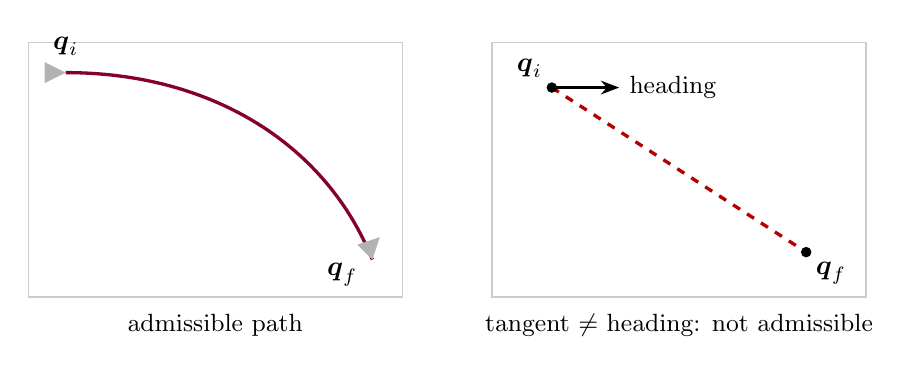
\begin{tikzpicture}[>=Stealth,scale=0.95]
  % left: admissible
  \draw[gray!40] (0,0) rectangle (5,3.4);
  \draw[very thick,purple!70!black] (0.5,3) .. controls (2.5,3) and (4,2) .. (4.6,0.5);
  \fill[gray!60] (0.5,3) -- ++(-0.28,0.14) -- ++(0,-0.28) -- cycle;
  \node at (0.5,3.35) {$\qi$};
  \fill[gray!60] (4.6,0.5) -- ++(0.1,0.3) -- ++(-0.3,-0.1) -- cycle;
  \node at (4.2,0.3) {$\qf$};
  \node[below] at (2.5,-0.1) {\small admissible path};
  % right: not admissible (straight line vs heading)
  \begin{scope}[xshift=6.2cm]
  \draw[gray!40] (0,0) rectangle (5,3.4);
  \draw[very thick,dashed,red!70!black] (0.8,2.8) -- (4.2,0.6);
  \draw[->,thick] (0.8,2.8) -- ++(0.9,0) node[right] {\small heading};
  \fill (0.8,2.8) circle (2pt) node[above left] {$\qi$};
  \fill (4.2,0.6) circle (2pt) node[below right] {$\qf$};
  \node[below] at (2.5,-0.1) {\small tangent $\ne$ heading: not admissible};
  \end{scope}
\end{tikzpicture}
\caption{A unicycle-like robot starting along the horizontal direction can follow a smooth curve that bends toward
$\qf$ (left), but not the straight segment (right), whose tangent disagrees with the heading at $\qi$.}
\end{figure}

\begin{intuition}
Think of parking a car: you cannot simply draw the straight line from where you are to the target spot, because the
car cannot move sideways. The planner must hand the robot a curve it is \emph{capable} of tracking.
Obstacles are deliberately left out here; the whole difficulty already lives in the nonholonomic constraints.
\end{intuition}

% =====================================================================
\section{Space-time separation \emph{(slide 4)}}

\begin{definition}[Path, timing law, trajectory]
A configuration-space \emph{trajectory} $\q(t)$, $t\in[t_i,t_f]$, with $\q(t_i)=\qi$ and $\q(t_f)=\qf$, can be split into:
\begin{itemize}[nosep]
\item a geometric \emph{path} $\q(s)$, where $s$ is a path parameter running from $s_i=s(t_i)$ to $s_f=s(t_f)$;
\item a \emph{timing law} $s=s(t)$, strictly monotonic (increasing).
\end{itemize}
One possible choice of $s$ is the arc length.
\end{definition}

\begin{itemize}
\item \textbf{Path planning:} plan an admissible path from $\qi$ to $\qf$.
\item \textbf{Trajectory planning:} plan an admissible trajectory from $\qi$ to $\qf$. It can be
\emph{direct}, or \emph{indirect}: first plan a path, then add a timing law.
\end{itemize}

\begin{figure}[h]
\centering
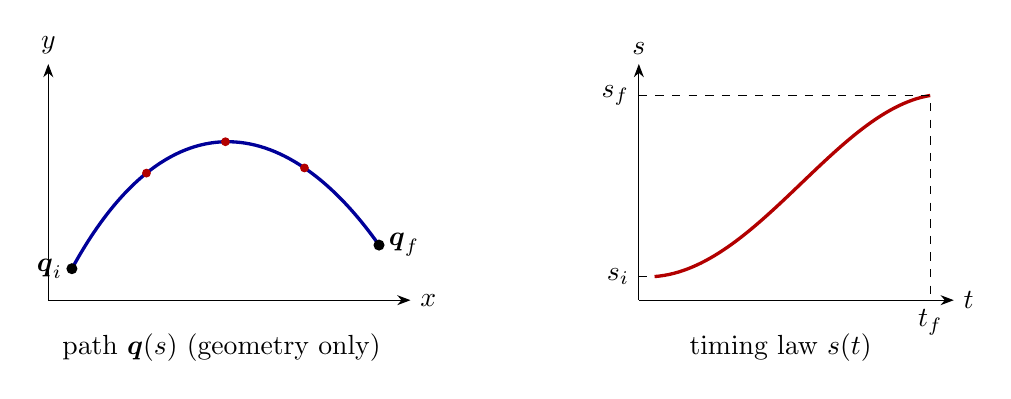
\begin{tikzpicture}[>=Stealth]
  % path
  \draw[->] (0,0) -- (4.6,0) node[right] {$x$};
  \draw[->] (0,0) -- (0,3) node[above] {$y$};
  \draw[very thick,blue!60!black] (0.3,0.4) .. controls (1.5,2.6) and (3,2.4) .. (4.2,0.7);
  \fill (0.3,0.4) circle (2pt) node[left] {$\qi$};
  \fill (4.2,0.7) circle (2pt) node[right] {$\qf$};
  \foreach \p in {0.25,0.5,0.75} {
    \pgfmathsetmacro{\bx}{(1-\p)^3*0.3+3*(1-\p)^2*\p*1.5+3*(1-\p)*\p^2*3+\p^3*4.2}
    \pgfmathsetmacro{\by}{(1-\p)^3*0.4+3*(1-\p)^2*\p*2.6+3*(1-\p)*\p^2*2.4+\p^3*0.7}
    \fill[red!70!black] (\bx,\by) circle (1.6pt);}
  \node at (2.2,-0.6) {path $\q(s)$ (geometry only)};
  % timing law
  \begin{scope}[xshift=7.5cm]
  \draw[->] (0,0) -- (4,0) node[right] {$t$};
  \draw[->] (0,0) -- (0,3) node[above] {$s$};
  \draw[very thick,red!70!black] (0.2,0.3) .. controls (1.5,0.4) and (2.5,2.4) .. (3.7,2.6);
  \draw[dashed] (0,0.3) node[left] {$s_i$} -- (0.2,0.3);
  \draw[dashed] (0,2.6) node[left] {$s_f$} -- (3.7,2.6) -- (3.7,0) node[below] {$t_f$};
  \node at (1.8,-0.6) {timing law $s(t)$};
  \end{scope}
\end{tikzpicture}
\caption{Space-time separation: the same path (left) can be run with many timing laws (right). The dots on the path
are equally spaced in $s$, hence equally spaced in time only when $s(t)$ is linear.}
\end{figure}

\begin{intuition}
A path is the \emph{railway track}, the timing law is the \emph{timetable}. The same track can be traveled quickly or
slowly, but the track itself decides whether the train can follow it at all. This is why a robot that cannot track a given
curve cannot be rescued by changing speed.
\end{intuition}

\paragraph{In symbols.} A trajectory $\q(t)$, $t\in[t_i,t_f]$, with $\q(t_i)=\qi$ and $\q(t_f)=\qf$, is rewritten as the
composition $\q(t)\;\to\;\q(s(t))$. The first factor, $\q(s)$ with $s\in[s_i,s_f]$, is the \emph{path}: it carries only the
\emph{geometry} of the motion. The second factor, $s(t)$ with $t\in[t_i,t_f]$, is the \emph{timing law}: it says \emph{when} each
point of the path is reached.

% =====================================================================
\section{Admissible paths and geometric model \emph{(slides 5--8)}}

\subsection{Geometric path admissibility \emph{(slides 5--6)}}

Intuitively, the local mobility limitation caused by the nonholonomic constraints also shows up on \emph{paths}: if a
motion is not admissible, speeding up or slowing down will not make it admissible. To see this, start from the
space-time separation:
\begin{equation}
\dot{\q}=\frac{\dd\q}{\dd t}=\frac{\dd\q}{\dd s}\,\dot s=\q'\,\dot s,
\label{eq:sep}
\end{equation}
where the prime denotes differentiation with respect to $s$. The vector $\q'$ is directed as the \emph{tangent} to the
path in configuration space, and $\dot s$ only changes its modulus.

\begin{example}[Tangent vector and arc length]\label{ex:arc}
Let $\mathcal C=\mathbb R^2$, with coordinates $(q_1,q_2)=(x,y)$, and consider the path
\[
x(s)=\sqrt{1-s^2},\qquad y(s)=s,\qquad s\in[0,1],
\]
a quarter of the unit circle going from $\qi=(1,0)$ to $\qf=(0,1)$. The tangent vector is
\[
\q'(s)=\begin{pmatrix}x'(s)\\ y'(s)\end{pmatrix}=\begin{pmatrix}-s/\sqrt{1-s^2}\\ 1\end{pmatrix},\qquad
\|\q'(s)\|=\frac{1}{\sqrt{1-s^2}}\ne 1 ,
\]
so this parameter $s$ is \emph{not} the arc length (for which one would have $\|\q'\|=1$, e.g., $x=\cos\sigma$, $y=\sin\sigma$).
\end{example}

\begin{figure}[H]
\centering
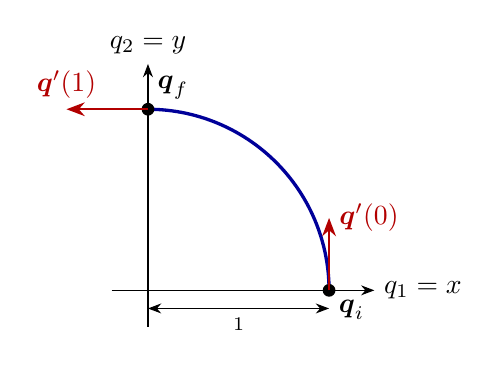
\begin{tikzpicture}[>=Stealth,scale=2.3]
  \draw[->] (-0.2,0) -- (1.25,0) node[right] {$q_1=x$};
  \draw[->] (0,-0.2) -- (0,1.25) node[above] {$q_2=y$};
  \draw[very thick,blue!60!black,domain=0:90,samples=60] plot ({cos(\x)},{sin(\x)});
  \fill (1,0) circle (1pt) node[below right] {$\qi$};
  \fill (0,1) circle (1pt) node[above right] {$\qf$};
  \draw[->,thick,red!70!black] (1,0) -- (1,0.4) node[right] {$\q'(0)$};
  \draw[->,thick,red!70!black] (0,1) -- (-0.45,1) node[above] {$\q'(1)$};
  \draw[<->] (0,-0.1) -- (1,-0.1) node[midway,below] {\scriptsize $1$};
\end{tikzpicture}
\caption{The path of Example~\ref{ex:arc}: the tangent direction is the same for any parametrization, only the modulus of $\q'$ depends on $s$.}
\end{figure}

\begin{intuition}
Reparametrizing a path (e.g., from $s$ to arc length $\sigma$) leaves the curve unchanged; it only rescales the tangent vector
$\q'$. This is why, in the geometric model, only the \emph{direction} of $\q'$ matters for admissibility, and why in all the planners
below we are free to use a convenient $s$ rather than the arc length.
\end{intuition}

\begin{proposition}[Geometric path admissibility]\label{prop:geoadm}
A path $\q(s)$ is the support of an admissible trajectory (for any timing law with $\dot s>0$) if and only if
\begin{equation}
A(\q)\,\q'=0 \qquad\text{at all points of the path.}
\end{equation}
\end{proposition}
\begin{proof}
Using \eqref{eq:sep}, the constraints become $A(\q)\dot{\q}=A(\q)\q'\,\dot s=0$. Since $\dot s(t)>0$ for all $t$ we may divide
by $\dot s$, which gives $A(\q)\q'=0$; conversely, if $A(\q)\q'=0$ holds along the path, then $A(\q)\dot\q=0$ for any
$\dot s$. \qedhere
\end{proof}

\begin{definition}[Geometric model and geometric inputs]
Let the columns of $G(\q)$ span $\Null(A(\q))$. All geometrically admissible paths are solutions of the
\emph{geometric model}
\begin{equation}
\q'=G(\q)\,\ut,
\end{equation}
where $\ut$ are the \emph{geometric inputs}. They are related to the velocity inputs of the kinematic model by
\begin{equation}
\boldsymbol{u}(t)=\ut(s)\,\dot s(t).
\end{equation}
\end{definition}

Once the geometric inputs $\ut(s)$ are chosen, the path is determined; selecting a timing law $s=s(t)$ then identifies a
particular trajectory along that path.

\paragraph{Kinematic versus geometric model.} The geometric model is built exactly in parallel to the kinematic model (KM).
Letting $\boldsymbol g_1,\dots,\boldsymbol g_m$ be the columns of $G(\q)$:
\begin{align}
\text{(KM)}\quad & A(\q)\dot\q=0\ \Rightarrow\ \dot\q\in\Null(A(\q))\ \Rightarrow\ \dot\q=\sum_{i=1}^m\boldsymbol g_i(\q)\,u_i,\\
\text{(GM)}\quad & A(\q)\q'=0\ \Rightarrow\ \q'\in\Null(A(\q))\ \Rightarrow\ \q'=\sum_{i=1}^m\boldsymbol g_i(\q)\,\tilde u_i .
\end{align}
Multiplying the geometric model by $\dot s$ and using $\dot\q=\q'\dot s$,
\[
\dot\q=\q'\,\dot s=\sum_{i=1}^m\boldsymbol g_i(\q)\,\tilde u_i\,\dot s ,
\]
and comparing with the kinematic model (the $\boldsymbol g_i$ are linearly independent) gives $u_i=\tilde u_i\,\dot s$. The $u_i$ are the
\emph{pseudovelocities} (or \emph{velocity inputs}); the $\tilde u_i$ are the \emph{geometric inputs}. In short: the kinematic model is a
\emph{trajectory generator}, the geometric model is a \emph{path generator}.


\begin{intuition}
The condition $A(\q)\q'=0$ is the kinematic model with time ``factored out''. The nonholonomic constraints say
which \emph{directions} of motion are allowed; speed has no say in direction. So the geometric model is just the
kinematic model run with a different clock: $s$ instead of $t$, and $\ut$ instead of $\boldsymbol u$.
\end{intuition}

\subsection{The unicycle example \emph{(slides 7--8)}}

For the unicycle the pure-rolling constraint is $\dot x\sin\theta-\dot y\cos\theta=0$, i.e., $(\sin\theta\;\;-\cos\theta\;\;0)\,\dot\q=0$. Replacing $\dot\q$ by $\q'\dot s$ and dividing by $\dot s>0$ gives $(\sin\theta\;\;-\cos\theta\;\;0)\,\q'=0$, the \emph{path admissibility} condition, which reads
\begin{equation}
x'\sin\theta-y'\cos\theta=0,
\end{equation}
i.e., the Cartesian path tangent must align with the sagittal axis of the robot. The robot may travel along the tangent in
either sense: forward motion if the heading points along the tangent, backward motion if it points opposite.

\begin{figure}[h]
\centering
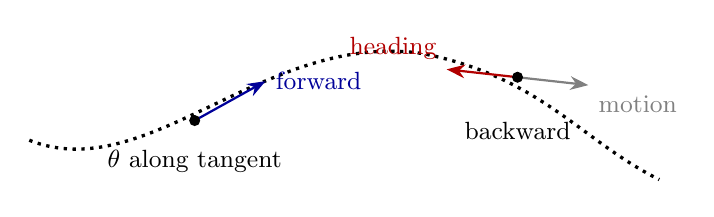
\begin{tikzpicture}[>=Stealth,
  robot/.style={circle,draw,minimum size=0.9cm}]
  \draw[dotted,very thick] (0,0.2) .. controls (1.5,-0.4) and (3,1.6) .. (5,1.3) .. controls (6.5,1.0) and (7,0.2) .. (8,-0.3);
  % forward robot at approx (2.2,0.55)
  \draw[thick,->,blue!60!black] (2.1,0.45) -- ++(0.9,0.5) node[right] {\small forward};
  \fill[black] (2.1,0.45) circle (2pt);
  \node[below] at (2.1,0.2) {\small $\theta$ along tangent};
  % backward robot
  \draw[thick,->,red!70!black] (6.2,1.0) -- ++(-0.9,0.1) node[above left] {\small heading};
  \draw[thick,->,gray] (6.2,1.0) -- ++(0.9,-0.1) node[below right] {\small motion};
  \fill[black] (6.2,1.0) circle (2pt);
  \node[below] at (6.2,0.55) {\small backward};
\end{tikzpicture}
\caption{Along a Cartesian path the unicycle heading is tangent to the path; it points the same way as the motion
(forward) or the opposite way (backward).}
\end{figure}

A Cartesian path with a \emph{discontinuous tangent} is not admissible, unless the unicycle is allowed to stop at the
discontinuity points to realign with the new tangent.

The geometric model of the unicycle is
\begin{align}
x'&=\vt\cos\theta,\nonumber\\
y'&=\vt\sin\theta,\\
\theta'&=\wt,\nonumber
\end{align}
with geometric inputs related to the velocity inputs by $v(t)=\vt(s)\,\dot s(t)$ and $\omega(t)=\wt(s)\,\dot s(t)$.
\begin{example}[A Cartesian path with a corner]\label{ex:corner}
Consider a Cartesian path made of a horizontal segment followed by a vertical one. Is it admissible for a unicycle? Two paths in
the configuration space $(x,y,\theta)$ have this same \emph{footprint} in the $(x,y)$ plane:
\begin{enumerate}[nosep,label=(\arabic*)]
\item $\theta$ stays at $0$ (or jumps at the corner). On the horizontal segment $y'=0$ and $x'\sin 0-y'\cos 0=0$ holds, but on the
vertical segment $x'=0$, $y'\ne0$ and the condition fails; a jump of $\theta$ would make the path discontinuous in $\mathcal C$.
\textbf{Not admissible.}
\item $\theta=0$ on the horizontal segment; at the corner $\theta$ goes from $0$ to $\pi/2$ while $x'=y'=0$ (rotation on the spot);
then $\theta=\pi/2$ on the vertical segment. The condition holds at every point, so the path \textbf{is admissible}, but only
if the unicycle \emph{stops} at the corner.
\end{enumerate}
\end{example}

\begin{figure}[H]
\centering
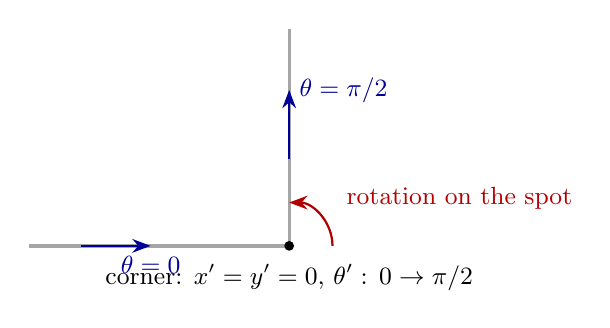
\begin{tikzpicture}[>=Stealth,scale=1.1]
  \draw[very thick,gray!70] (0,0) -- (3,0) -- (3,2.5);
  \draw[->,thick,blue!60!black] (0.6,0) -- (1.4,0) node[below] {\small $\theta=0$};
  \draw[->,thick,blue!60!black] (3,1.0) -- (3,1.8) node[right] {\small $\theta=\pi/2$};
  \draw[->,thick,red!70!black] (3.5,0) arc (0:90:0.5);
  \node[red!70!black,font=\small,anchor=west] at (3.55,0.55) {rotation on the spot};
  \fill (3,0) circle (1.6pt);
  \node[below] at (3,-0.1) {\small corner: $x'=y'=0$, $\theta':\,0\to\pi/2$};
\end{tikzpicture}
\caption{Path (2) of Example~\ref{ex:corner}: the footprint has a corner, but the robot realigns with the new tangent by rotating at the corner.}
\end{figure}
\begin{intuition}
A corner in the Cartesian path is a place where the robot would have to change heading instantly. A unicycle can do
that only by stopping and rotating on the spot, i.e., by ``cheating'' the pure path picture.
\end{intuition}

\paragraph{Planning formulation.} Path planning for WMRs is generally formulated and solved with the \emph{geometric}
model. Trajectory planning can be solved \emph{directly} with the kinematic model, or \emph{indirectly} by first planning a
geometric path and then choosing a timing law.

% =====================================================================
\section{Flat outputs \emph{(slides 9--13)}}

\subsection{Differential flatness \emph{(slides 9--10)}}

\begin{definition}[Differential flatness]
The system $\dot{\boldsymbol x}=f(\boldsymbol x)+G(\boldsymbol x)\boldsymbol u$ is \emph{differentially flat} if there exists a set of
outputs $\boldsymbol y$, called \emph{flat outputs}, such that the state and the control inputs can be expressed
\emph{algebraically} as functions of $\boldsymbol y$ and its time derivatives:
\begin{align}
\boldsymbol x&=\boldsymbol x\big(\boldsymbol y,\dot{\boldsymbol y},\ddot{\boldsymbol y},\dots,\boldsymbol y^{(r)}\big),\\
\boldsymbol u&=\boldsymbol u\big(\boldsymbol y,\dot{\boldsymbol y},\ddot{\boldsymbol y},\dots,\boldsymbol y^{(r)}\big).
\end{align}
\end{definition}

The definition applies equally to \emph{geometric} models if $s$ replaces $t$ and derivatives with respect to $t$ are
replaced by derivatives with respect to $s$. If the path (trajectory) of $\boldsymbol y$ is known, the path (trajectory) of
$\boldsymbol x$ and the history of $\boldsymbol u$ in $s$ (or $t$) can be \emph{reconstructed}.

\begin{intuition}
Flat outputs are ``free handles'': pick any sufficiently smooth curve for $\boldsymbol y$, and everything else follows by
differentiation, with no differential equation to integrate. For a unicycle, picking a smooth planar curve $(x(s),y(s))$ is
enough: the heading is the direction of the curve, and the inputs are its speed and curvature.
\end{intuition}

\begin{proposition}[Flatness of the unicycle and the bicycle]\label{prop:flatuni}
The unicycle and the bicycle are differentially flat with $x$ and $y$ as flat outputs. For the geometric model of the unicycle, a
Cartesian path $(x(s),y(s))$ determines the path of the whole state $\q(s)=(x(s),y(s),\theta(s))$ and the geometric inputs:
\begin{align}
\theta(s)&=\arctan\frac{y'(s)}{x'(s)}=\atan\big(y'(s),x'(s)\big)+k\pi,\\
\vt(s)&=\pm\sqrt{(x'(s))^2+(y'(s))^2},\\
\wt(s)&=\frac{y''(s)x'(s)-x''(s)y'(s)}{(x'(s))^2+(y'(s))^2}.
\end{align}
For forward (backward) motion take $k=1$ ($k=0$) and the $+$ ($-$) sign.
For the bicycle, let $L$ be the wheelbase and $delta$ the front-wheel steering angle; its kinematic model is
\begin{align*}
\dot x&=v\cos\theta, & \dot y&=v\sin\theta, &
\dot\theta&=\frac{v}{L}\tan\delta.
\end{align*}
On intervals where the vehicle does not stop, the same Cartesian outputs reconstruct its state and inputs as
\begin{align*}
\theta&=\operatorname{atan2}(\dot y,\dot x)\quad\text{(modulo $\pi$)},\\
v&=\pm\sqrt{\dot x^2+\dot y^2},\\
\delta&=\arctan\!\left(L\,\frac{\operatorname{sgn}(v)(\dot x\ddot y-\dot y\ddot x)}
                              {(\dot x^2+\dot y^2)^{3/2}}\right).
\end{align*}
The sign of $v$ selects forward or backward motion, with the corresponding heading branch.
\end{proposition}
\begin{proof}[Derivation for the unicycle]
From $x'=\vt\cos\theta$ and $y'=\vt\sin\theta$ we get $(x')^2+(y')^2=\vt^2$, hence $\vt=\pm\sqrt{(x')^2+(y')^2}$, and
$y'/x'=\tan\theta$, hence $\theta=\arctan(y'/x')$ up to a multiple of $\pi$. Differentiating $\tan\theta=y'/x'$:
\[
\frac{\theta'}{\cos^2\theta}=\frac{y''x'-x''y'}{(x')^2}\ \Longrightarrow\ 
\wt=\theta'=\frac{y''x'-x''y'}{(x')^2}\cos^2\theta=\frac{y''x'-x''y'}{(x')^2+(y')^2},
\]
since $\cos^2\theta=(x')^2/\big((x')^2+(y')^2\big)$. \qedhere
\end{proof}

\begin{proof}[Derivation for the bicycle]
The first two bicycle equations have the same form as the unicycle equations, so they give $v$ and $\theta$ directly
from $(x,y)$ and their first derivatives, as above. Differentiating the heading yields
\[
\dot\theta=\frac{\dot x\ddot y-\dot y\ddot x}{\dot x^2+\dot y^2}.
\]
Using $\dot\theta=(v/L)\tan\delta$ and $|v|=\sqrt{\dot x^2+\dot y^2}$ (with the heading branch chosen consistently
with the sign of $v$), we obtain
\[
\tan\delta=L\frac{\operatorname{sgn}(v)(\dot x\ddot y-\dot y\ddot x)}
                         {(\dot x^2+\dot y^2)^{3/2}},
\]
which gives the steering reconstruction above. Thus state and inputs are algebraic functions of the flat outputs and
their derivatives, proving flatness wherever $v\ne0$. \qedhere
\end{proof}

\begin{intuition}
$\vt$ is the ``speed along the curve'' and $\wt$ is $\vt$ times the \emph{curvature} of the Cartesian path: the formula for
$\wt$ is the familiar planar curvature formula $\kappa=(y''x'-x''y')/\big((x')^2+(y')^2\big)^{3/2}$ multiplied by $\vt$.
The sign choice only decides whether the robot runs the curve nose-first or tail-first.
\end{intuition}

\subsection{Flatness and the chained form \emph{(slides 11--12)}}

\begin{theorem}[Flatness, chained form, linearization]\label{thm:flat}
For driftless dynamic systems, differential flatness is a necessary and sufficient condition for transformability into
chained form; hence all WMRs with dimension up to 4 are flat. For general dynamic systems, differential flatness is a
necessary and sufficient condition for linearizability via dynamic feedback.
\end{theorem}

\paragraph{Singular points of the reconstruction.}
\begin{itemize}[nosep]
\item If $x'(s)=y'(s)=0$ at an isolated point (as at cusps or motion inversions), then $\vt(s)=0$ there; at these points $\theta(s)$ and $\wt(s)$ can be computed by continuity arguments.
\item The reconstruction of $\theta$ and $\wt$ \emph{fails} if the Cartesian path degenerates to a point ($x'(s)=y'(s)=0$ identically). In fact, the unicycle may then have any orientation at the contact point, and may even be rotating on the spot.
\end{itemize}

Geometrically: at an isolated cusp the Cartesian tangent vanishes only at the tip, so $\vt=0$ there, the robot stops, inverts its
motion and leaves along the other branch; if instead $x'\equiv y'\equiv0$ over an interval, the contact point does not move and
$\theta,\wt$ cannot be recovered from $(x,y)$ (they are free in the geometric model $\theta'=\wt$).

\begin{figure}[H]
\centering
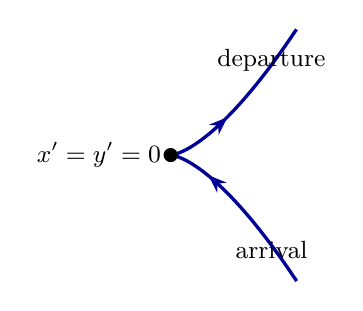
\begin{tikzpicture}[>=Stealth,scale=1.6]
  \draw[very thick,blue!60!black,smooth,domain=-1:1,samples=50] plot ({\x*\x},{\x*\x*\x});
  \fill (0,0) circle (1.6pt) node[left] {\small $x'=y'=0$};
  \draw[->,thick,blue!60!black] (0.45,-0.30) -- (0.30,-0.16);
  \draw[->,thick,blue!60!black] (0.30,0.16) -- (0.45,0.30);
  \node[font=\small] at (0.8,-0.75) {arrival};
  \node[font=\small] at (0.8,0.75) {departure};
\end{tikzpicture}
\caption{A cusp of the Cartesian path: the tangent vanishes only at the tip, where the unicycle inverts its motion.}
\end{figure}

\begin{proposition}[Flatness of the $(2,n)$ chained form]
The $(2,n)$ chained form is differentially flat, with flat outputs $z_1$ and $z_n$; all the other state variables and the
associated control inputs can be computed from them.
\end{proposition}

\begin{example}[The $(2,3)$ chained form]\label{ex:chain23}
Consider
\begin{align}
z_1'&=\wwt_1,\nonumber\\
z_2'&=\wwt_2,\\
z_3'&=z_2\,\wwt_1.\nonumber
\end{align}
The reconstruction formulas are
\begin{equation}
z_2=\frac{z_3'}{z_1'}\quad\text{(state)},\qquad
\wwt_1=z_1',\qquad
\wwt_2=\frac{z_1'z_3''-z_1''z_3'}{(z_1')^2}\quad\text{(input)}.
\end{equation}
\end{example}
\begin{proof}[Derivation]
The first equation gives $\wwt_1=z_1'$. Substituting in the third, $z_3'=z_2z_1'$, so $z_2=z_3'/z_1'$ (when $z_1'\ne0$).
The second equation then gives $\wwt_2=z_2'=\big(z_3''z_1'-z_3'z_1''\big)/(z_1')^2$ by the quotient rule. \qedhere
\end{proof}

\begin{intuition}
In chained form the first variable $z_1$ acts as ``clock'': it advances at the rate $\wwt_1$. Dividing the third equation by
the first, $\dd z_3/\dd z_1=z_2$: the slope of $z_3$ against $z_1$ \emph{is} $z_2$. Choose the curve $z_3(z_1)$ and
$z_2$ is forced; its derivative then gives the remaining input. This is exactly the same ``choose the curve, read off the rest''
mechanism as for $(x,y)$ in the unicycle.
\end{intuition}

\subsection{An algorithm for planning with flat outputs \emph{(slide 13)}}

Reconstruction formulas associate admissible paths (trajectories) to the evolution of the flat outputs, which can be chosen
\emph{arbitrarily}. This leads to the following algorithm.

\begin{algorithm}[Path planning via flat outputs]\label{alg:flat}
\begin{enumerate}[nosep,label=\arabic*.]
\item Compute $\boldsymbol y_i$ and $\boldsymbol y_f$ corresponding to $\qi$ and $\qf$.
\item Find $\boldsymbol y(s)$ by interpolating $\boldsymbol y_i$ and $\boldsymbol y_f$ with the appropriate boundary conditions for $\q$.
\item Use the reconstruction formulas to find $\q(s)$ and $\ut(s)$.
\end{enumerate}
\end{algorithm}

The resulting path is \emph{automatically} admissible, i.e., it satisfies the nonholonomic constraints at all points. The same
algorithm can be used for \emph{trajectory planning} by interpolating over $t$ rather than over $s$.

\begin{figure}[h]
\centering
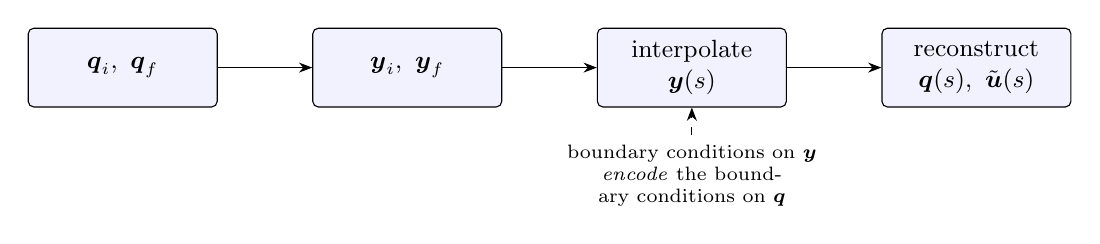
\begin{tikzpicture}[>=Stealth,node distance=1.2cm,
  blk/.style={draw,rounded corners=2pt,fill=blue!5,minimum height=1.0cm,minimum width=2.4cm,align=center,font=\small}]
  \node[blk] (a) {$\qi,\ \qf$};
  \node[blk,right=of a] (b) {$\boldsymbol y_i,\ \boldsymbol y_f$};
  \node[blk,right=of b] (c) {interpolate\\ $\boldsymbol y(s)$};
  \node[blk,right=of c] (d) {reconstruct\\ $\q(s),\ \ut(s)$};
  \draw[->] (a) -- (b); \draw[->] (b) -- (c); \draw[->] (c) -- (d);
  \node[font=\scriptsize,above=1pt of $(b)!0.5!(c)$] {\ };
  \node[font=\scriptsize,below=0.35cm of c,text width=3.6cm,align=center] (n) {boundary conditions on $\boldsymbol y$ \\ \emph{encode} the boundary conditions on $\q$};
  \draw[->,dashed] (n) -- (c);
\end{tikzpicture}
\caption{Planning with flat outputs: admissibility is built into the reconstruction step.}
\end{figure}

\begin{intuition}
Normally planning for a nonholonomic robot means solving a constrained problem. Flatness turns it into an
\emph{unconstrained} one: the constraints are already ``absorbed'' by the reconstruction formulas. The only subtlety is that
orientation (and higher-order variables) are \emph{not} flat outputs, so their boundary values must be translated into
\emph{derivative} conditions on $\boldsymbol y$; this is the role of the ``appropriate boundary conditions'' in step 2.
\end{intuition}

% =====================================================================
\section{Unicycle path planning via Cartesian polynomials \emph{(slides 14--15)}}
We apply Algorithm~\ref{alg:flat} to the unicycle, whose flat outputs are $x$ and $y$. Given $\qi=(x_i,y_i,\theta_i)$ and
$\qf=(x_f,y_f,\theta_f)$, find an admissible path $\q(s)$, $s\in[s_i,s_f]$, with $\q(s_i)=\qi$ and $\q(s_f)=\qf$.

Let $s_i=0$, $s_f=1$ and use \emph{pre-fitted cubic polynomials}
\begin{align}
x(s)&=s^3x_f-(s-1)^3x_i+\alpha_x s^2(s-1)+\beta_x s(s-1)^2,\\
y(s)&=s^3y_f-(s-1)^3y_i+\alpha_y s^2(s-1)+\beta_y s(s-1)^2,
\end{align}
which already satisfy the boundary conditions on $x,y$ (indeed $x(0)=x_i$, $x(1)=x_f$). Since $\theta_i$ and $\theta_f$ are
given, we must also impose
\begin{equation}
\arctan\frac{y'(0)}{x'(0)}=\theta_i,\qquad \arctan\frac{y'(1)}{x'(1)}=\theta_f .
\end{equation}
Since the interpolation is done independently in $x$ and $y$, these are separated as
\begin{equation}
\begin{aligned}
x'(0)&=k_i\cos\theta_i, & x'(1)&=k_f\cos\theta_f,\\
y'(0)&=k_i\sin\theta_i, & y'(1)&=k_f\sin\theta_f,
\end{aligned}
\end{equation}
where $k_i\ne0$, $k_f\ne0$ are free parameters.
In other words, the flat outputs of the boundary configurations are $(x_i,y_i)$ and $(x_f,y_f)$, while the orientations $\theta_i,\theta_f$ translate into conditions on the first derivatives. Each of $x(s)$ and $y(s)$ thus carries four boundary conditions (value and derivative at both ends), which matches the four coefficients of a cubic.

\begin{proposition}[Cartesian cubic planner]\label{prop:cart}
Under the simplifying assumption $k_i=k_f=k$, the additional boundary conditions give
\begin{equation}
\begin{aligned}
\alpha_x&=k\cos\theta_f-3x_f, & \beta_x&=k\cos\theta_i+3x_i,\\
\alpha_y&=k\sin\theta_f-3y_f, & \beta_y&=k\sin\theta_i+3y_i.
\end{aligned}
\end{equation}
Moreover $\vt(0)=\vt(1)=k$; $k>0$ gives forward motion, $k<0$ backward motion.
\end{proposition}
\begin{proof}
Differentiating,
$x'(s)=3s^2x_f-3(s-1)^2x_i+\alpha_x(3s^2-2s)+\beta_x\big((s-1)^2+2s(s-1)\big)$. Then $x'(0)=-3x_i+\beta_x=k\cos\theta_i$ and
$x'(1)=3x_f+\alpha_x=k\cos\theta_f$, which give $\beta_x,\alpha_x$. The computation for $y$ is identical. At the extremes
$\vt=\pm\sqrt{(x')^2+(y')^2}=\pm|k|$, with the sign of $k$ for the chosen direction of motion. \qedhere
\end{proof}

From $x(s)$ and $y(s)$ one obtains $\theta(s)$, $\vt(s)$ and $\wt(s)$ via the reconstruction formulas of
Proposition~\ref{prop:flatuni}.

\begin{intuition}
This is cubic \emph{Hermite interpolation}: $(x_i,y_i)$ and $(x_f,y_f)$ are the endpoints, and the vectors
$k(\cos\theta_i,\sin\theta_i)$ and $k(\cos\theta_f,\sin\theta_f)$ are the end tangents. The heading is forced to be tangent to
the path (so the path is admissible), and $k$ is a ``tangent length'': a large $k$ makes the robot leave $\qi$ and arrive at
$\qf$ \emph{straight and for a long stretch} before bending in the middle, a small $k$ gives a more direct, tighter curve.
\end{intuition}

\begin{example}[Worked numbers: forward parking]\label{ex:fwd}
Take $\qi=(0,0,0)$ and $\qf=(4,-3,-\pi/2)$. Then $\alpha_x=-12$, $\beta_x=k$, $\alpha_y=9-k$, $\beta_y=0$, so
\[
x(s)=(k-8)s^3+(12-2k)s^2+ks,\qquad y(s)=(6-k)s^3-(9-k)s^2 .
\]
One checks $x'(0)=k$, $y'(0)=0$ (heading $0$, speed $k$) and $x'(1)=0$, $y'(1)=-k$ (heading $-\pi/2$, speed $k$).
At the start, $\wt(0)=y''(0)/k=2(k-9)/k$: for $k=5$ this is $-1.6$ (the robot immediately steers right), whereas for $k=20$ it is
$+1.1$ (the robot first swings slightly \emph{left}, up, and then comes down).
\end{example}

\begin{intuition}
The sign change of $\wt(0)$ at $k=9$ is the numerical face of ``long tangents overshoot'': with a very large $k$ the cubic is
stretched along the initial heading, so it first bulges forward and upward before turning down to the target.
\end{intuition}

\begin{figure}[h]
\centering
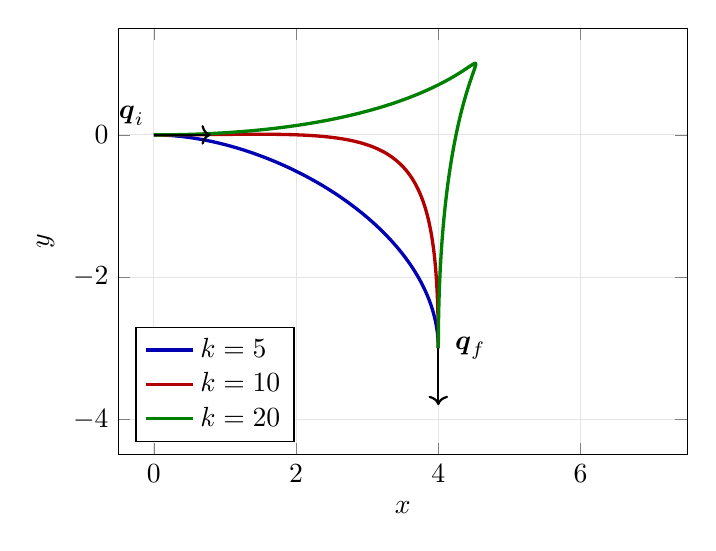
\begin{tikzpicture}
\begin{axis}[width=0.78\textwidth,height=7cm,axis equal image,xlabel={$x$},ylabel={$y$},
  grid=both,grid style={gray!20},legend pos=south west,legend cell align=left,
  xmin=-0.5,xmax=7.5,ymin=-4.5,ymax=1.5]
  \addplot[blue!70!black,very thick,domain=0:1,samples=120]
    ({4*x*x*x-12*x*x*(x-1)+5*x*(x-1)*(x-1)},{-3*x*x*x+(9-5)*x*x*(x-1)});
  \addplot[red!70!black,very thick,domain=0:1,samples=120]
    ({4*x*x*x-12*x*x*(x-1)+10*x*(x-1)*(x-1)},{-3*x*x*x+(9-10)*x*x*(x-1)});
  \addplot[green!50!black,very thick,domain=0:1,samples=120]
    ({4*x*x*x-12*x*x*(x-1)+20*x*(x-1)*(x-1)},{-3*x*x*x+(9-20)*x*x*(x-1)});
  \legend{$k=5$,$k=10$,$k=20$}
  \draw[->,thick] (axis cs:0,0) -- (axis cs:0.8,0);
  \draw[->,thick] (axis cs:4,-3) -- (axis cs:4,-3.8);
  \node[anchor=south east] at (axis cs:0,0) {$\qi$};
  \node[anchor=west] at (axis cs:4.1,-3) {$\qf$};
\end{axis}
\end{tikzpicture}
\caption{Cartesian cubic planner for the forward-parking problem of Example~\ref{ex:fwd}, for increasing $k$
(own computation from the formulas above). Larger $k$ produces longer take-off and landing phases.}
\end{figure}

% =====================================================================
\section{Unicycle path planning via the chained form \emph{(slides 16--17)}}

As an alternative one may transform the unicycle into the $(2,3)$ chained form, whose flat outputs are $z_1$ and $z_3$.
(The standard unicycle transformation is $z_1=\theta$, $z_2=x\cos\theta+y\sin\theta$, $z_3=x\sin\theta-y\cos\theta$, with inputs
$w_1=\omega$, $w_2=v-z_3\omega$.)

First compute the initial and final values of $z_1,z_2,z_3$ corresponding to $\qi$ and $\qf$. Then, assuming
$z_{1,i}\ne z_{1,f}$, define $z_1$ and $z_3$ over $[0,1]$ as
\begin{align}
z_1(s)&=z_{1,f}\,s-(s-1)\,z_{1,i},\\
z_3(s)&=s^3z_{3,f}-(s-1)^3z_{3,i}+\alpha_3s^2(s-1)+\beta_3s(s-1)^2,
\end{align}
which already satisfy the boundary conditions on $z_1,z_3$. Since $z_{2,i}$ and $z_{2,f}$ are also given, we must impose
\begin{equation}
\frac{z_3'(0)}{z_1'(0)}=z_{2,i},\qquad \frac{z_3'(1)}{z_1'(1)}=z_{2,f}.
\end{equation}

\begin{proposition}[Chained-form cubic planner]
Imposing these conditions gives
\begin{equation}
\alpha_3=z_{2,f}(z_{1,f}-z_{1,i})-3z_{3,f},\qquad
\beta_3=z_{2,i}(z_{1,f}-z_{1,i})+3z_{3,i}.
\end{equation}
\end{proposition}
\begin{proof}
$z_1'(s)=z_{1,f}-z_{1,i}=:\Delta$ is constant. As in Proposition~\ref{prop:cart},
$z_3'(0)=-3z_{3,i}+\beta_3$ and $z_3'(1)=3z_{3,f}+\alpha_3$; setting them equal to $z_{2,i}\Delta$ and $z_{2,f}\Delta$ respectively
gives the result. \qedhere
\end{proof}

From $z_1(s)$ and $z_3(s)$ one obtains $z_2(s)$ and $\wwt_1(s)$, $\wwt_2(s)$ via the reconstruction formulas of
Example~\ref{ex:chain23}. Finally $\q(s)$, $\vt(s)$ and $\wt(s)$ are computed by inverting the chained form coordinate and
input transformations.

\paragraph{The singular case.} If $z_{1,i}=z_{1,f}$ (i.e., $\theta_i=\theta_f$) the construction breaks down ($z_1$ would be
constant). One can introduce a \emph{via point} $\q_v=(x_v,y_v,\theta_v)$ with $\theta_v\ne\theta_i$ and split the original problem
in two; alternatively, set $z_{1,f}=z_{1,i}+2\pi$ (a full turn).

\paragraph{Direct trajectory planning.} Both previous schemes (Cartesian polynomials and chained form) can be used for direct
trajectory planning: just let $s=t$ and use the kinematic model.

\begin{intuition}
Here $z_1=\theta$ is used as the interpolation ``clock'' and it moves \emph{linearly} between $\theta_i$ and $\theta_f$:
the heading changes monotonically. That is why $\theta_i=\theta_f$ is a problem: the clock does not move at all and the curve
$z_3(z_1)$ has nothing to be a function of. Adding a via point or a full $2\pi$ turn restores a clock that ticks.
\end{intuition}

\paragraph{Remark on the numerical results.} For the unicycle chained form, the position enters $z_2,z_3$ through
the current $(x,y)$. Placing the origin of $z_2,z_3$ at $\qi$ (so that $z_{2,i}=z_{3,i}=0$) changes the plan: with the global origin a
reorientation generates a Cartesian displacement, whereas with the origin at $\qi$ pure rotations on the spot are
representable (in the numerical check for $\qi=(1,1,0)\to\qf=(1,1,\pi/2)$ with origin at $\qi$ the integration gives $c_0=c_1=0$, i.e.
$x\equiv y\equiv$ const).

% =====================================================================
\section{Path planning via parametrized inputs \emph{(slides 18--21)}}

\subsection{Chained form with parametrized inputs \emph{(slides 18--20)}}

A different approach, not directly based on flatness, consists in writing the inputs in \emph{parametrized form} and then
imposing that the robot goes from $\qi$ to $\qf$. Assume the robot can be put in chained form,
\begin{align}
z_1'&=\wwt_1,\nonumber\\
z_2'&=\wwt_2,\nonumber\\
z_3'&=z_2\wwt_1,\\
&\ \,\vdots\nonumber\\
z_n'&=z_{n-1}\wwt_1,\nonumber
\end{align}
which becomes \emph{linear} (hence easily integrable) if $\wwt_1(s)$ is constant.

Let $\Delta=z_{1,f}-z_{1,i}$ and choose the geometric inputs for $s\in[s_i,s_f]=[0,|\Delta|]$ as
\begin{align}
\wwt_1&=\sign(\Delta),\\
\wwt_2&=c_0+c_1s+\dots+c_{n-2}s^{n-2}.
\end{align}
Integrating the chained-form equations from $\boldsymbol z(0)=\boldsymbol z_i$ and imposing $\boldsymbol z(|\Delta|)=\boldsymbol z_f$ leads to a
\emph{linear system}
\begin{equation}
D(\Delta)\begin{pmatrix}c_0\\c_1\\\vdots\\c_{n-2}\end{pmatrix}=\boldsymbol d(\boldsymbol z_i,\boldsymbol z_f,\Delta),
\end{equation}
with $D(\Delta)$ invertible if $\Delta\ne0$.

\begin{proposition}[The $(2,3)$ case]
For the $(2,3)$ chained form,
\begin{equation}
D=\begin{pmatrix}|\Delta|&\dfrac{\Delta^2}{2}\\[6pt]\sign(\Delta)\dfrac{\Delta^2}{2}&\dfrac{\Delta^3}{6}\end{pmatrix},\qquad
\boldsymbol d=\begin{pmatrix}z_{2,f}-z_{2,i}\\ z_{3,f}-z_{3,i}-z_{2,i}\Delta\end{pmatrix},
\end{equation}
and $\det D=-\sign(\Delta)\,\Delta^4/12\ne0$ whenever $\Delta\ne0$.
\end{proposition}
\begin{proof}
With $\wwt_1=\sign(\Delta)$, $\wwt_2=c_0+c_1s$: $z_1(s)=z_{1,i}+\sign(\Delta)s$, which reaches $z_{1,f}$ at $s=|\Delta|$;
$z_2(s)=z_{2,i}+c_0s+c_1s^2/2$; and $z_3'=\sign(\Delta)z_2$ gives
$z_3(s)=z_{3,i}+\sign(\Delta)\big(z_{2,i}s+c_0s^2/2+c_1s^3/6\big)$. Imposing $z_2(|\Delta|)=z_{2,f}$ gives
$c_0|\Delta|+c_1\Delta^2/2=z_{2,f}-z_{2,i}$. Imposing $z_3(|\Delta|)=z_{3,f}$ and using $\sign(\Delta)|\Delta|=\Delta$,
$\sign(\Delta)|\Delta|^3=\Delta^3$ gives
$\sign(\Delta)\tfrac{\Delta^2}{2}c_0+\tfrac{\Delta^3}{6}c_1=z_{3,f}-z_{3,i}-z_{2,i}\Delta$.
Finally $\det D=|\Delta|\Delta^3/6-\sign(\Delta)\Delta^4/4=-\sign(\Delta)\Delta^4/12$. \qedhere
\end{proof}

If $\Delta=0$ ($z_{1,i}=z_{1,f}$) a singular case is met, which can be handled as before (e.g., with a via point). Once planning
on the chained form is complete, $\q(s)$ and $\ut(s)$ for the original model are computed via the inverse coordinate and
input transformations. Although this method does not make explicit use of flat outputs, it still relies on transformability in chained form,
which is strongly related to flatness (Theorem~\ref{thm:flat}).

\begin{intuition}
With $\wwt_1$ constant, $s$ simply counts how far the ``clock'' variable $z_1$ has advanced, and the remaining equations are a
\emph{chain of integrators} driven by the polynomial $\wwt_2$. The $n-1$ unknown coefficients are exactly as many as the
$n-1$ boundary conditions on $z_2,\dots,z_n$ (those on $z_1$ are met by the choice of the interval $[0,|\Delta|]$), so a
square linear system results. For $n=3$ there are two coefficients $(c_0,c_1)$ for two conditions.
\end{intuition}

\subsection{Other parametrizations and trajectory planning \emph{(slide 21)}}

Other classes of parametrized inputs can be used, such as sinusoidal and piecewise-constant functions. Note that in
\emph{all} the presented path planning methods the path parameter $s$ \emph{does not represent the arc length}. This scheme too can
be used for direct trajectory planning by replacing $s$ with $t$ and using the kinematic model in place of the geometric model.

% =====================================================================
\section{Parking a unicycle: numerical results \emph{(slides 22--27)}}

\subsection{Planner based on Cartesian polynomials \emph{(slides 22--24)}}

\begin{itemize}
\item \textbf{Forward parking} ($k=5>0$): the motion is forward; a negative $k$ would produce a backward motion. There are no motion inversions (a general result for this planner).
\item \textbf{Effect of $k$:} increasing $k$ (e.g., $k=10$ and $k=20$) leads to elongated take-off and landing phases; still no motion inversions.
\item \textbf{Parallel parking} and \textbf{reorientation} (again $k=10$ and $k=20$): since the planner is based on flat outputs, a Cartesian path of \emph{finite length} is needed for \emph{any} kind of reconfiguration.
\end{itemize}

\begin{figure}[H]
\centering
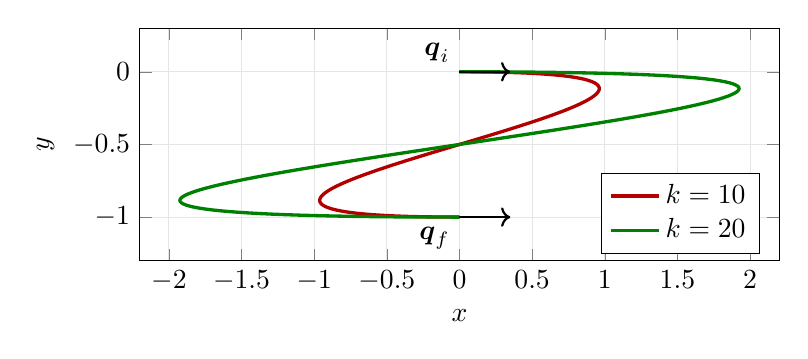
\begin{tikzpicture}
\begin{axis}[width=0.8\textwidth,height=6.5cm,axis equal image,xlabel={$x$},ylabel={$y$},grid=both,grid style={gray!20},
  legend pos=south east,legend cell align=left,xmin=-2.2,xmax=2.2,ymin=-1.3,ymax=0.3]
  \addplot[red!70!black,very thick,domain=0:1,samples=120] ({10*x*(x-1)*(2*x-1)},{2*x*x*x-3*x*x});
  \addplot[green!50!black,very thick,domain=0:1,samples=120] ({20*x*(x-1)*(2*x-1)},{2*x*x*x-3*x*x});
  \legend{$k=10$,$k=20$}
  \draw[->,thick] (axis cs:0,0) -- (axis cs:0.35,0);
  \draw[->,thick] (axis cs:0,-1) -- (axis cs:0.35,-1);
  \node[anchor=south east] at (axis cs:0,0) {$\qi$};
  \node[anchor=north east] at (axis cs:0,-1) {$\qf$};
\end{axis}
\end{tikzpicture}
\caption{Parallel parking with the Cartesian planner, $\qi=(0,0,0)\to\qf=(0,-1,0)$ (own computation). A larger $k$ widens the
forward and backward excursions needed to shift sideways.}
\end{figure}

\begin{figure}[H]
\centering
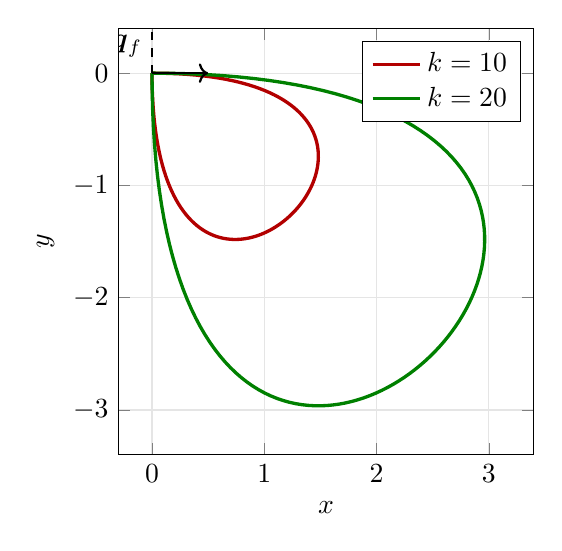
\begin{tikzpicture}
\begin{axis}[width=0.7\textwidth,height=7cm,axis equal image,xlabel={$x$},ylabel={$y$},grid=both,grid style={gray!20},
  legend pos=north east,legend cell align=left,xmin=-0.3,xmax=3.4,ymin=-3.4,ymax=0.4]
  \addplot[red!70!black,very thick,domain=0:1,samples=120] ({10*x*(x-1)*(x-1)},{10*x*x*(x-1)});
  \addplot[green!50!black,very thick,domain=0:1,samples=120] ({20*x*(x-1)*(x-1)},{20*x*x*(x-1)});
  \legend{$k=10$,$k=20$}
  \draw[->,thick] (axis cs:0,0) -- (axis cs:0.5,0);
  \draw[->,thick,dashed] (axis cs:0,0) -- (axis cs:0,0.5);
  \node[anchor=south east] at (axis cs:0,0.05) {$\qi,\ \qf$};
\end{axis}
\end{tikzpicture}
\caption{Reorientation $\qi=(0,0,0)\to\qf=(0,0,\pi/2)$ with the Cartesian planner (own computation): the robot leaves heading east
(solid arrow), draws a finite loop and returns heading north (dashed arrow).}
\end{figure}

\begin{intuition}
Reorienting a unicycle in place is easy for the physical robot (rotate on the spot), but the Cartesian planner has no way to say
``stay at a point''. The reconstruction formulas fail when the Cartesian path degenerates to a point (Section 4), so the planner must
draw a small loop in the plane to change orientation.
\end{intuition}

\subsection{Planner based on parametrized inputs \emph{(slides 25--27)}}

\begin{itemize}
\item \textbf{Forward parking:} the first maneuver is similar to that of the other planner. In the second maneuver a \emph{cusp} appears: this planner can only generate paths along which the orientation varies monotonically.
\item \textbf{Parallel parking:} the problem is solved with a via point, or by imposing a full rotation.
\item \textbf{Reorientation:} using the classical chained form transformation, a Cartesian displacement is generated; placing the origin of $z_2,z_3$ at $\qi$ avoids it.
\end{itemize}

\begin{figure}[H]
\centering
\begin{minipage}{0.49\textwidth}\centering
\begin{tikzpicture}
\begin{axis}[width=\linewidth,axis equal image,xlabel={$x$},ylabel={$y$},grid=both,grid style={gray!20},
  xmin=-1,xmax=1,ymin=-1.3,ymax=0.3]
  \addplot[blue!70!black,very thick] table[x=x,y=y] {par_via1.dat};
  \addplot[orange!85!black,very thick] table[x=x,y=y] {par_via2.dat};
  \fill (axis cs:0,0) circle (1.5pt) node[above right] {\scriptsize $\qi$};
  \fill (axis cs:0,-0.5) circle (1.5pt) node[left] {\scriptsize $\q_v$};
  \fill (axis cs:0,-1) circle (1.5pt) node[below right] {\scriptsize $\qf$};
\end{axis}
\end{tikzpicture}

\small with a via point
\end{minipage}
\begin{minipage}{0.49\textwidth}\centering
\begin{tikzpicture}
\begin{axis}[width=\linewidth,axis equal image,xlabel={$x$},ylabel={$y$},grid=both,grid style={gray!20},
  xmin=-1,xmax=1,ymin=-1.3,ymax=0.7]
  \addplot[blue!70!black,very thick] table[x=x,y=y] {par_2pi.dat};
  \fill (axis cs:0,0) circle (1.5pt) node[above right] {\scriptsize $\qi$};
  \fill (axis cs:0,-1) circle (1.5pt) node[below right] {\scriptsize $\qf$};
\end{axis}
\end{tikzpicture}

\small imposing a full rotation ($z_{1,f}=z_{1,i}+2\pi$)
\end{minipage}
\caption{Parallel parking $\qi=(0,0,0)\to\qf=(0,-1,0)$ with the parametrized-input planner. Since $\theta_i=\theta_f$ ($\Delta=0$), the
problem is either split at a via point (here $\q_v=(0,-0.5,-\pi/4)$) or solved with a full rotation of the orientation (own computation).}
\end{figure}

\begin{figure}[H]
\centering
\begin{minipage}{0.49\textwidth}\centering
\begin{tikzpicture}
\begin{axis}[width=\linewidth,height=6cm,xlabel={$x$},ylabel={$y$},grid=both,grid style={gray!20},
  xmin=4.88,xmax=5.04,ymin=-0.02,ymax=0.14]
  \addplot[blue!70!black,very thick] table[x=x,y=y] {reor_glob.dat};
  \fill (axis cs:5,0) circle (1.5pt) node[below right] {\scriptsize $\qi,\ \qf$};
\end{axis}
\end{tikzpicture}

\small classical transformation (origin of $z_2,z_3$ elsewhere)
\end{minipage}
\begin{minipage}{0.49\textwidth}\centering
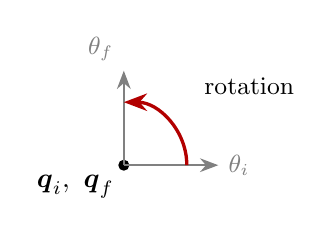
\begin{tikzpicture}[>=Stealth]
  \fill (0,0) circle (2pt) node[below left] {$\qi,\ \qf$};
  \draw[->,thick,gray] (0,0) -- (1.2,0) node[right] {\small $\theta_i$};
  \draw[->,thick,gray] (0,0) -- (0,1.2) node[above left] {\small $\theta_f$};
  \draw[->,very thick,red!70!black] (0.8,0) arc (0:90:0.8);
  \node[font=\small,anchor=west] at (0.9,1.0) {rotation};
\end{tikzpicture}

\small origin of $z_2,z_3$ placed at $\qi$
\end{minipage}
\caption{Reorientation $\qi=(x,y,0)\to\qf=(x,y,\pi/2)$ with the parametrized-input planner (own computation). With the classical
transformation a small Cartesian displacement is generated (note the scale of the axes); placing the origin at $\qi$ gives $c_0=c_1=0$,
i.e., a pure rotation on the spot.}
\end{figure}

\begin{figure}[h]
\centering
\begin{tikzpicture}
\begin{axis}[width=0.78\textwidth,height=7cm,axis equal image,xlabel={$x$},ylabel={$y$},
  grid=both,grid style={gray!20},legend pos=south west,legend cell align=left,
  xmin=-0.5,xmax=7.5,ymin=-4.5,ymax=1.5]
  \addplot[blue!70!black,very thick,domain=0:1,samples=120]
    ({4*x*x*x-12*x*x*(x-1)+5*x*(x-1)*(x-1)},{-3*x*x*x+(9-5)*x*x*(x-1)});
  \addplot[orange!85!black,very thick,dashed] table[x=x,y=y] {fwd_chained.dat};
  \legend{Cartesian cubic ($k=5$),chained form with parametrized $\wwt_2$}
  \draw[->,thick] (axis cs:0,0) -- (axis cs:0.8,0);
  \draw[->,thick] (axis cs:4,-3) -- (axis cs:4,-3.8);
  \node[anchor=south east] at (axis cs:0,0) {$\qi$};
  \node[anchor=west] at (axis cs:4.1,-3) {$\qf$};
\end{axis}
\end{tikzpicture}
\caption{The two planners on the same forward-parking problem $\qi=(0,0,0)\to\qf=(4,-3,-\pi/2)$ (own computation).
The parametrized-input planner turns monotonically from $0$ to $-\pi/2$ with $\wt=\pm1$ per unit of $s$, so $s$ is the angle swept, not the arc length.}
\end{figure}

% =====================================================================
% =====================================================================
\section{Choice of timing law \emph{(slides 28--30)}}
 
\subsection{Choosing $s(t)$ \emph{(slide 28)}}
 
Once a configuration-space path $\q(s)$, $s\in[s_i,s_f]$, has been generated, obtaining a trajectory requires choosing a
\emph{timing law}
\begin{equation}
s=s(t),\qquad t\in[t_i,t_f],\qquad s(t_i)=s_i,\quad s(t_f)=s_f .
\end{equation}
Typically $t_f$ is \emph{not} assigned a priori: it results from the timing law itself. Two simple choices are
\begin{itemize}[nosep]
\item a \emph{constant} $\dot s$ over $[t_i,t_f]$, i.e., a \emph{linear} timing law;
\item a \emph{trapezoidal} $\dot s$, i.e., a \emph{quadratic--linear--quadratic} timing law.
\end{itemize}
Whatever the choice, it must be \emph{feasible}: the resulting velocities must comply with the robot velocity bounds.
 
Given a geometric path $\q(s)$ with inputs $\ut(s)$, any $s=s(t)$ with $\dot s>0$ yields an admissible trajectory with inputs
$v(t)=\vt(s)\dot s$, $\omega(t)=\wt(s)\dot s$. For a unicycle with bounds $|v|\le v_{\max}$, $|\omega|\le\omega_{\max}$, feasibility means
\[
\dot s(t)\le\min\left\{\frac{v_{\max}}{|\vt(s)|},\ \frac{\omega_{\max}}{|\wt(s)|}\right\}\qquad\text{for all } t .
\]
 
\begin{intuition}
The trapezoidal $\dot s$ is the familiar ``accelerate, cruise, decelerate'' profile: $s(t)$ is a parabola, then a straight line, then a
parabola, so the robot starts and stops without jumps in $\dot s$. The linear law is the cruise phase alone. Slowing down scales
\emph{both} inputs by the same factor, so the shape of the path never changes; it is the sharp parts of the path (large $|\wt|$) that
force the robot to slow down.
\end{intuition}
 
\subsection{Linear timing law for a unicycle with velocity bounds \emph{(slides 29--30)}}
 
Consider a unicycle subject to bounds on the velocity inputs, and assume that a path $\q(s)$ has been generated, with geometric
inputs $\vt(s)$ and $\wt(s)$. Choose the linear timing law
\begin{equation}
s=\frac{t}{k},\qquad t\in[0,t_f],\qquad t_f=k\,s_f ,
\end{equation}
(taking $s_i=0$). Since $\dot s=1/k$,
\begin{equation}
v(t)=\frac{\vt(s(t))}{k},\qquad \omega(t)=\frac{\wt(s(t))}{k}.
\end{equation}
 
\begin{proposition}[Feasible linear timing law]\label{prop:timing}
Let
\[
\vt_{\mathrm{peak}}=\max_{s\in[s_i,s_f]}|\vt(s)|,\qquad \wt_{\mathrm{peak}}=\max_{s\in[s_i,s_f]}|\wt(s)| .
\]
The linear timing law is feasible if and only if $k\ge \max\{\vt_{\mathrm{peak}}/v_{\max},\,\wt_{\mathrm{peak}}/\omega_{\max}\}$, and
the feasible choice with the shortest duration $t_f=ks_f$ is
\begin{equation}
k=\max\left\{\frac{\vt_{\mathrm{peak}}}{v_{\max}},\ \frac{\wt_{\mathrm{peak}}}{\omega_{\max}}\right\}.
\end{equation}
With this $k$, either $v$ or $\omega$ saturates at (at least) one instant of time.
\end{proposition}
\begin{proof}
$|v(t)|\le v_{\max}$ for all $t$ is equivalent to $\max_s|\vt(s)|/k\le v_{\max}$, i.e., $k\ge\vt_{\mathrm{peak}}/v_{\max}$; likewise
$|\omega(t)|\le\omega_{\max}$ for all $t$ is equivalent to $k\ge\wt_{\mathrm{peak}}/\omega_{\max}$. Both hold iff $k$ is at least the larger
of the two ratios, and since $t_f=ks_f$ the smallest such $k$ gives the shortest duration. For that $k$ one of the two inequalities
is an equality, so the corresponding input reaches its bound at the instant where $|\vt|$ or $|\wt|$ attains its peak. \qedhere
\end{proof}
 
\begin{example}[Worked numbers]
Let $s_f=1$, $\vt_{\mathrm{peak}}=2$, $\wt_{\mathrm{peak}}=1.5$, $v_{\max}=0.5$, $\omega_{\max}=0.6$ (consistent units). Then
$k=\max\{2/0.5,\ 1.5/0.6\}=\max\{4,\ 2.5\}=4$, so $t_f=4$; the peak linear velocity is $2/4=0.5=v_{\max}$ (saturated), while the
peak angular velocity is $1.5/4=0.375<\omega_{\max}$.
\end{example}
 
\begin{intuition}
Dividing both geometric inputs by the same $k$ is like playing the same film in slow motion: the path is unchanged and every
velocity shrinks by the factor $1/k$. We slow down just enough so that the most demanding point of the path, in terms of
$v$ or of $\omega$, exactly touches its bound. That is why one input saturates: slowing down any further would be feasible but wasteful.
\end{intuition}
 
More generally, any choice of a constant $k\ne1$ based on feasibility or optimality arguments can be seen as a \emph{uniform time
scaling} with respect to the straightforward choice $s=t$ (which corresponds to $k=1$).
% =====================================================================
\section{Summary}

\begin{table}[h]
\centering
\small
\renewcommand{\arraystretch}{1.25}
\begin{tabular}{@{}p{3.2cm}p{3.7cm}p{3.7cm}p{3.7cm}@{}}
\toprule
 & \textbf{Cartesian polynomials} & \textbf{Chained form (cubic $z_3$)} & \textbf{Parametrized inputs}\\
\midrule
Flat outputs used & $x,\ y$ & $z_1,\ z_3$ & not directly (needs chained form)\\
What is chosen & cubic $x(s),y(s)$; $k$ free & $z_1$ linear, $z_3$ cubic & $\wwt_1=\sign\Delta$, $\wwt_2$ polynomial\\
Unknowns & $\alpha_x,\beta_x,\alpha_y,\beta_y$ (closed form), $k$ & $\alpha_3,\beta_3$ (closed form) & $c_0,\dots,c_{n-2}$ (linear system $D\boldsymbol c=\boldsymbol d$)\\
Singular case & --- & $\theta_i=\theta_f$ & $\Delta=0$\\
Singular case remedy & --- & via point or $+2\pi$ & via point or $+2\pi$\\
Orientation & follows the Cartesian curve & monotonic & monotonic\\
Cusps & none & may appear & may appear\\
$s$ is arc length? & no & no & no\\
Direct trajectory planning & $s=t$ & $s=t$ & $s=t$\\
\bottomrule
\end{tabular}
\caption{Comparison of the three planners for the unicycle (all assume obstacle-free motion).}
\end{table}

\begin{figure}[h]
\centering
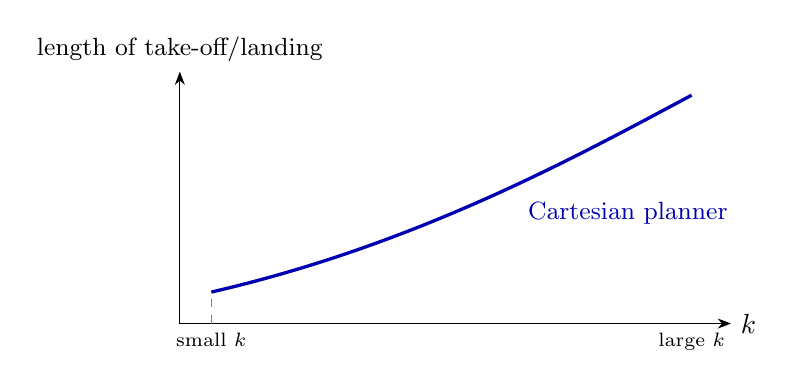
\begin{tikzpicture}[>=Stealth]
  \draw[->] (0,0) -- (7,0) node[right] {$k$};
  \draw[->] (0,0) -- (0,3.2) node[above] {\small length of take-off/landing};
  \draw[very thick,blue!70!black] (0.4,0.4) .. controls (3,1.0) and (5,2.1) .. (6.5,2.9);
  \node[blue!70!black,font=\small,anchor=west] at (4.3,1.4) {Cartesian planner};
  \draw[dashed,gray] (0.4,0) -- (0.4,0.4);
  \node[below,font=\scriptsize] at (0.4,0) {small $k$};
  \node[below,font=\scriptsize] at (6.5,0) {large $k$};
\end{tikzpicture}
\caption{Qualitative trade-off in the Cartesian planner: larger $k$ gives longer straight take-off and landing phases and
a possible initial overshoot (qualitative sketch, not measured data).}
\end{figure}

\subsection*{Key take-aways}
\begin{itemize}
\item A path is admissible for a nonholonomic WMR iff $A(\q)\q'=0$; this is independent of the timing law, which only
converts a path into a trajectory ($\boldsymbol u=\ut\,\dot s$).
\item Differentially flat systems (unicycle, bicycle, all WMRs up to dimension 4) can be planned by interpolating the flat outputs
and reconstructing the rest: admissibility comes for free.
\item For the unicycle, a cubic Cartesian Hermite curve with tangent length $k$ gives a closed-form planner; the sign of $k$ selects
forward or backward motion and a large $k$ elongates take-off and landing.
\item In chained form, either interpolate $z_1,z_3$ or parametrize $\wwt_2$ and solve a linear system; both fail when
$\theta_i=\theta_f$ and need a via point or a $2\pi$ turn, and both produce monotonically varying orientation.
\item In none of the methods does $s$ represent the arc length, and every scheme becomes a direct trajectory planner by
setting $s=t$.
\end{itemize}

\end{document}